\chapter{Figures and Tables of Part 1}
\label{app:part1}

This appendix contains all figures and tables of Part~1. They are referred to from the answers in the main text.

\section{Assignment 1: Closed Section A}
\label{app:a1}

\begin{figure}[H]
    \centering
    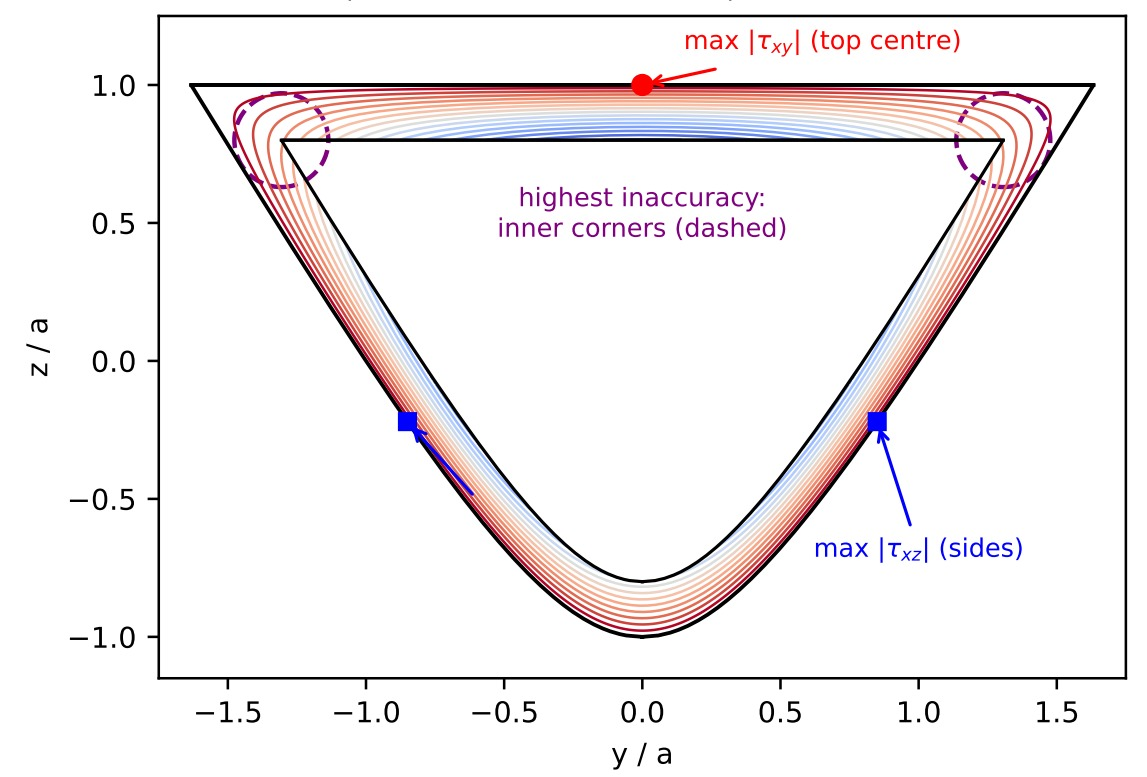
\includegraphics[width=0.95\linewidth]{figures/A1_prandtl (2).jpeg}
    \caption{Contours of the Prandtl stress function in the wall of section A (based on Figure~4 of the assignment, $k=0.8$). Marked are the locations of maximum $|\tau_{xy}|$ and $|\tau_{xz}|$ (Question~\ref{sec:a1-1}) and the regions with the highest inaccuracy (dashed, Question~\ref{sec:a1-2}).}
    \label{fig:a1-prandtl}
\end{figure}

\begin{figure}[H]
    \centering
    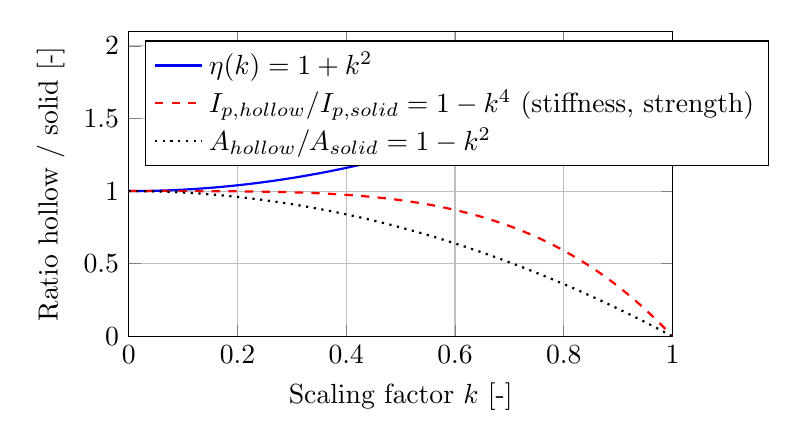
\begin{tikzpicture}
        \begin{axis}[
            width=0.7\textwidth,
            height=0.45\textwidth,
            xlabel={Scaling factor $k$ [-]},
            ylabel={Ratio hollow / solid [-]},
            xmin=0, xmax=1,
            ymin=0, ymax=2.1,
            grid=major,
            legend pos=north west,
            legend cell align=left,
            domain=0:1,
            samples=100,
        ]
            \addplot[thick, blue] {1 + x^2};
            \addlegendentry{$\eta(k) = 1+k^2$}
            \addplot[thick, red, dashed] {1 - x^4};
            \addlegendentry{$I_{p,hollow}/I_{p,solid} = 1-k^4$ (stiffness, strength)}
            \addplot[thick, black, dotted] {1 - x^2};
            \addlegendentry{$A_{hollow}/A_{solid} = 1-k^2$}
        \end{axis}
    \end{tikzpicture}
    \caption{Cross-sectional efficiency $\eta(k)$ and the relative stiffness, strength and area of the hollow section as a function of $k$.}
    \label{fig:efficiency}
\end{figure}

\section{Assignment 2: Open Sections B}
\label{app:a2}

\begin{table}[H]
  \centering\small
  \caption{Plate thicknesses of the half section (from the legends of Figures~5 and~6).}
  \label{tab:B1B2}
  \begin{tabular}{llcc}
    \toprule
    Plate & Position & B1 & B2 \\
    \midrule
    centre girder (half)      & $y=0$, $0<z<a$          & $2t_p$   & $2t_p$ \\
    bottom plating            & $0<y<2.5a$              & $3t_p$   & $3t_p$ \\
    bottom, bilge, side shell & $y>2.5a$ up to the deck & $2t_p$   & $2t_p$ \\
    inner bottom              & $0<y<4a$, $z=a$         & $2t_p$   & $3t_p$ \\
    longitudinal bulkhead     & $y=2.5a$, $0<z<5a$      & $2.5t_p$ & $t_p$  \\
    deck                      & $2.5a<y<4a$, $z=5a$     & $3t_p$   & $3t_p$ \\
    side girder               & $y=a$, $0<z<a$          & --       & $3t_p$ \\
    stringer deck             & $2.5a<y<4a$, $z=3a$     & --       & $t_p$  \\
    \bottomrule
  \end{tabular}
\end{table}

\begin{figure}[H]
    \centering
    \begin{tikzpicture}[scale=1.3, >={Stealth[length=2.2mm,width=1.8mm]},
        cell/.style={circle, draw, inner sep=1pt, minimum size=4.6mm,
                     font=\footnotesize, fill=white},
        dim/.style={thin, {Latex[length=1.6mm,width=1.2mm]}-{Latex[length=1.6mm,width=1.2mm]}},
        ext/.style={very thin, gray}]

        % \flow{x}{y}{dx}{dy}{q}: arrow at (x,y) in direction (dx,dy), thickness ~ q,
        % plus the mirrored arrow in the port half
        \def\flow#1#2#3#4#5{%
            \pgfmathsetmacro{\lw}{max(0.4,#5/0.0331*2.4)}%
            \draw[->, red!75!black, line width=\lw pt]
                ({#1-0.2*(#3)},{#2-0.2*(#4)}) -- ({#1+0.2*(#3)},{#2+0.2*(#4)});
            \draw[->, red!75!black, line width=\lw pt]
                ({-(#1)-0.2*(#3)},{#2+0.2*(#4)}) -- ({-(#1)+0.2*(#3)},{#2-0.2*(#4)});
        }

        % ---------------- structure (starboard half, mirrored to port) ----------------
        \foreach \s in {1,-1}{
            \begin{scope}[xscale=\s]
                \draw[line width=1pt] (0,0) -- (3.5,0) arc (-90:0:0.5) -- (4,5) -- (2.5,5) -- (2.5,0);
                \draw[line width=1pt] (0,1) -- (4,1);   % inner bottom
                \draw[line width=1pt] (2.5,3) -- (4,3); % stringer deck
                \draw[line width=1pt] (1,0) -- (1,1);   % side girder
            \end{scope}
        }
        \draw[line width=2pt] (0,0) -- (0,1);           % centre girder
        \draw[dashed, gray] (0,-0.3) -- (0,5.3) node[above, black] {\small C.L.};

        % applied torque (counter-clockwise)
        \draw[->, thick] (0,3) ++(-30:0.6) arc (-30:210:0.6);
        \node at (0,3) {$M_t$};

        % ---------------- shear flow arrows ----------------
        % bottom shell
        \flow{0.5}{0}{1}{0}{0.0331}
        \flow{1.75}{0}{1}{0}{0.0315}
        \flow{3.0}{0}{1}{0}{0.0285}
        % inner bottom
        \flow{0.5}{1}{-1}{0}{0.0331}
        \flow{1.75}{1}{-1}{0}{0.0315}
        \flow{3.25}{1}{-1}{0}{0.0060}
        % girders in the double bottom
        \flow{1}{0.5}{0}{1}{0.0016}
        \flow{2.5}{0.5}{0}{1}{0.0030}
        % side shell
        \flow{4}{0.75}{0}{1}{0.0285}
        \flow{4}{2}{0}{1}{0.0225}
        \flow{4}{4}{0}{1}{0.0203}
        % inner side wall of the wing tanks
        \flow{2.5}{2}{0}{-1}{0.0225}
        \flow{2.5}{4}{0}{-1}{0.0203}
        % stringer deck and deck
        \flow{3.25}{3}{-1}{0}{0.0022}
        \flow{3.25}{5}{-1}{0}{0.0203}

        % ---------------- cell numbers ----------------
        \foreach \x/\y/\n in {0.5/0.5/1, 1.75/0.5/2, 2.8/0.5/3, 3.25/2/4, 3.25/4/5}{
            \node[cell] at (\x,\y) {\n};                          % starboard
            \node[cell, draw=gray, text=gray] at (-\x,\y) {\n};   % port (mirror)
        }

        % ---------------- bilge radius ----------------
        \fill (3.5,0.5) circle (0.8pt);
        \draw[thin, -{Latex[length=1.4mm,width=1mm]}] (3.5,0.5) -- ({3.5+0.5*cos(-45)},{0.5+0.5*sin(-45)});
        \node[font=\scriptsize, anchor=south] at (3.5,0.52) {$r=0.5a$};

        % ---------------- horizontal dimensions ----------------
        \foreach \x/\ytop in {0/-0.05, 1/-0.05, 2.5/-0.05, 4/0.4}{
            \draw[ext] (\x,\ytop) -- (\x,-0.65);
        }
        \draw[dim] (0,-0.5)   -- node[below, font=\small] {$a$}    (1,-0.5);
        \draw[dim] (1,-0.5)   -- node[below, font=\small] {$1.5a$} (2.5,-0.5);
        \draw[dim] (2.5,-0.5) -- node[below, font=\small] {$1.5a$} (4,-0.5);

        % ---------------- vertical dimensions ----------------
        \foreach \y/\xl in {0/3.55, 1/4.05, 3/4.05, 5/4.05}{
            \draw[ext] (\xl,\y) -- (5.0,\y);
        }
        \draw[dim] (4.9,0) -- node[right, font=\small] {$a$}  (4.9,1);
        \draw[dim] (4.9,1) -- node[right, font=\small] {$2a$} (4.9,3);
        \draw[dim] (4.9,3) -- node[right, font=\small] {$2a$} (4.9,5);
    \end{tikzpicture}
    \caption{Shear flow in design B2 for a counter-clockwise torque $M_t$. The arrow
    thickness is proportional to the magnitude of the shear flow. The cells are
    numbered 1--5 on both sides; the port cells (grey) are the mirror image of the
    starboard cells and carry the same shear flow, so there is no net shear flow
    through the centre girder.}
    \label{fig:shearflow-B2}
\end{figure}

\begin{table}[H]
  \centering
  \caption{Net shear flow and shear stress per wall for design B2.}
  \label{tab:B2walls}
  \begin{tabular}{llcc}
    \toprule
    Wall & $t$ & $q_{net}$ [$M_t/a^2$] & $\tau = q_{net}/t$ [$M_t/(a^2t_p)$] \\
    \midrule
    Centre girder                           & $4t_p$ & $q_1-q_1 = 0$             & $0$ \\
    Bottom and inner bottom, cell 1         & $3t_p$ & $q_1 = 0.0331$            & $0.0110$ \\
    Side girder                             & $3t_p$ & $q_1-q_2 = 0.0016$        & $0.0005$ \\
    Bottom and inner bottom, cell 2         & $3t_p$ & $q_2 = 0.0315$            & $0.0105$ \\
    Bulkhead in double bottom               & $t_p$  & $q_2-q_3 = 0.0030$        & $0.0030$ \\
    Bottom, bilge and side shell, cell 3    & $2t_p$ & $q_3 = 0.0285$            & $0.0143$ \\
    Inner bottom under wing tank            & $3t_p$ & $q_3-q_4 = 0.0060$        & $0.0020$ \\
    Side shell, cell 4                      & $2t_p$ & $q_4 = 0.0225$            & $0.0113$ \\
    \textbf{Bulkhead, cell 4}               & $\boldsymbol{t_p}$ & $\boldsymbol{q_4 = 0.0225}$ & $\boldsymbol{0.0225}$ \\
    Stringer deck                           & $t_p$  & $q_4-q_5 = 0.0022$        & $0.0022$ \\
    Side shell, cell 5                      & $2t_p$ & $q_5 = 0.0203$            & $0.0102$ \\
    Bulkhead, cell 5                        & $t_p$  & $q_5 = 0.0203$            & $0.0203$ \\
    Deck                                    & $3t_p$ & $q_5 = 0.0203$            & $0.0068$ \\
    \bottomrule
  \end{tabular}
\end{table}

\begin{figure}[H]
    \centering
    \begin{tikzpicture}[scale=0.75, >={Stealth[length=2.2mm,width=1.8mm]},
        pt/.style={circle, draw, inner sep=1pt, minimum size=4.6mm,
                   font=\footnotesize, fill=white},
        dim/.style={thin, {Latex[length=1.6mm,width=1.2mm]}-{Latex[length=1.6mm,width=1.2mm]}},
        ext/.style={very thin, gray}]

        \pgfmathsetmacro{\ee}{1.672}   % e = 1.672a

        % ---------------- structure (line width ~ plate thickness) ----------------
        \draw[line width=1.4pt] (-4,5) -- (-4,0);                 % port side,  t_sp
        \draw[line width=1.4pt] ( 4,5) -- ( 4,0);                 % stb side,   t_sp
        \draw[line width=2.6pt, line cap=rect] (-4,0) -- (4,0);   % bottom,     t_bp
        \draw[dashed, gray] (0,-2.0) -- (0,5.4) node[above, black] {\small C.L.};

        % ---------------- contour points ----------------
        \node[pt] at (-4, 5.55)     {1};
        \node[pt] at (-4.55,-0.55)  {2};
        \node[pt] at ( 0.5, 0.5)    {3};
        \node[pt] at ( 4.55,-0.55)  {4};
        \node[pt] at ( 4, 5.55)     {5};

        % ---------------- z = e (omega = 0 on the sides) ----------------
        \foreach \s in {-1,1} \draw[thin] ({\s*3.8},\ee) -- ({\s*4.2},\ee);
        \node[font=\scriptsize, right] at (-3.8,\ee) {$z=e$};

        % ---------------- shear centre / pole ----------------
        \fill[red!70!black] (0,-\ee) circle (2.2pt);
        \node[right, font=\small, red!70!black] at (0.1,-\ee) {CT};

        % ---------------- thickness labels ----------------
        \node[left,  font=\small] at (-4.1,2.8) {$t_{sp}$};
        \node[below, font=\small] at (-2,-0.1)  {$t_{bp}$};

        % ---------------- dimension e ----------------
        \draw[ext] (0,-\ee) -- (-0.85,-\ee);
        \draw[dim] (-0.7,0) -- node[left, font=\small] {$e$} (-0.7,-\ee);

        % ---------------- dimension A ----------------
        \foreach \x in {-4,4} \draw[ext] (\x,-0.15) -- (\x,-2.55);
        \draw[dim] (-4,-2.4) -- node[below, font=\small] {$A = 8a$} (4,-2.4);

        % ---------------- dimension B ----------------
        \foreach \y in {0,5} \draw[ext] (4.15,\y) -- (5.15,\y);
        \draw[dim] (5.0,0) -- node[right, font=\small] {$B = 5a$} (5.0,5);

        % ---------------- coordinate system ----------------
        \draw[->] (-6.2,-1.8) -- (-5.4,-1.8) node[right, font=\small] {$y$};
        \draw[->] (-6.2,-1.8) -- (-6.2,-1.0) node[above, font=\small] {$z$};
    \end{tikzpicture}
    \caption{U-shaped section of design BU ($A=8a$, $B=5a$, $t_{sp}=3.5t_p$,
             $t_{bp}=6.5t_p$) with contour points 1--5 and twist centre CT at a
             distance $e=1.672a$ below the bottom plate.}
    \label{fig:BU_section}
\end{figure}

\begin{figure}[H]
  \centering
  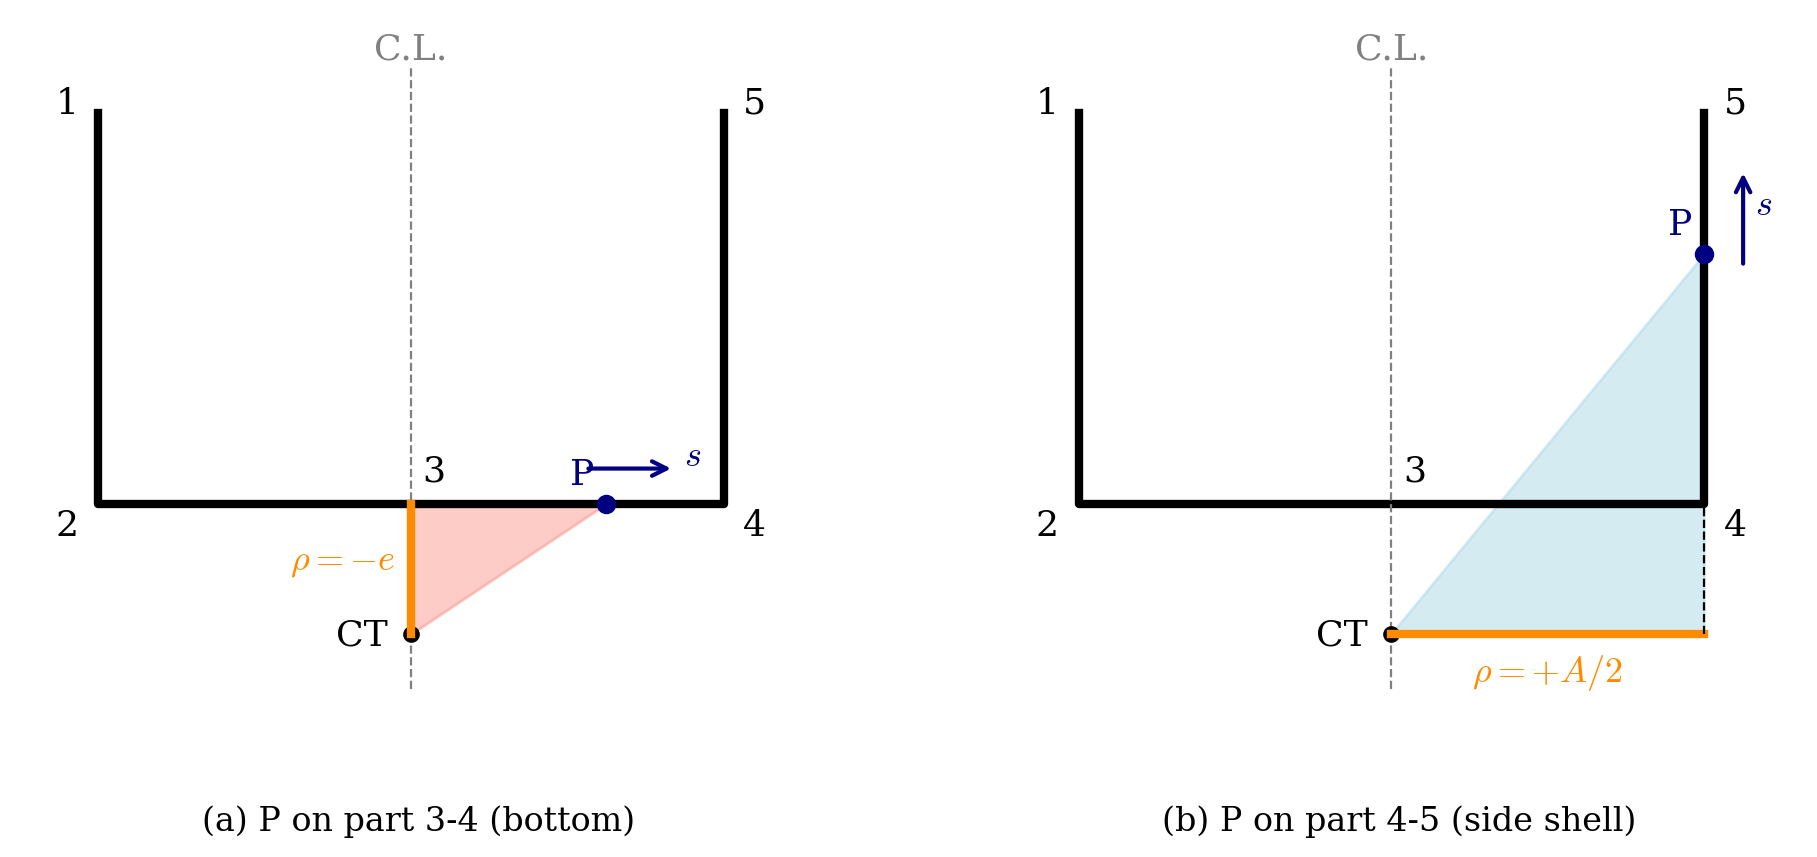
\includegraphics[width=0.9\textwidth]{figures/rho_figuur}
  \caption{Definition of $\rho$ for the U-shaped section BU. Left: P on the bottom
    plate (part 3--4), $\rho=-e$. Right: P on the side shell (part 4--5),
    $\rho=+A/2$.}
  \label{fig:rho}
\end{figure}

\begin{figure}[H]
    \centering
    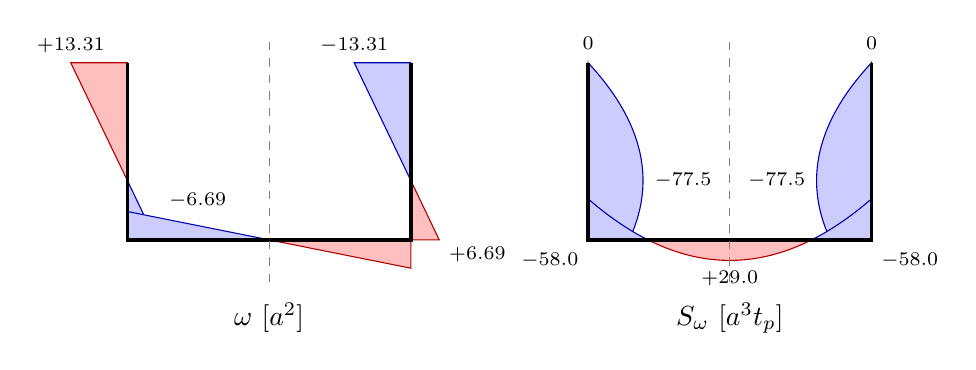
\begin{tikzpicture}[scale=0.45,
        posfill/.style={fill=red!25, draw=red!70!black, thin},
        negfill/.style={fill=blue!20, draw=blue!70!black, thin},
        val/.style={font=\scriptsize}]

        \pgfmathsetmacro{\ee}{1.672}

        % ================= sectorial coordinate omega =================
        \begin{scope}
            \filldraw[posfill] (-4,5) -- (-5.6,5) -- (-4,\ee) -- cycle;   % port, upper
            \filldraw[negfill] (-4,\ee) -- (-3.2,0) -- (-4,0) -- cycle;   % port, lower
            \filldraw[negfill] (4,5) -- (2.4,5) -- (4,\ee) -- cycle;      % stb, upper
            \filldraw[posfill] (4,\ee) -- (4.8,0) -- (4,0) -- cycle;      % stb, lower
            \filldraw[negfill] (-4,0) -- (-4,0.8) -- (0,0) -- cycle;      % bottom, port
            \filldraw[posfill] (0,0) -- (4,-0.8) -- (4,0) -- cycle;       % bottom, stb

            \draw[line width=1.2pt] (-4,5) -- (-4,0) -- (4,0) -- (4,5);
            \draw[dashed, gray] (0,-1.2) -- (0,5.6);

            \node[val, above] at (-5.6,5) {$+13.31$};
            \node[val, above] at (2.4,5)  {$-13.31$};
            \node[val, right] at (-3.1,1.1) {$-6.69$};
            \node[val, right] at (4.8,-0.4) {$+6.69$};
            \node at (0,-2.2) {$\omega$ [$a^2$]};
        \end{scope}

        % ================= sectorial area moment S_omega =================
        \begin{scope}[shift={(13,0)}]
            % port side shell (all negative, plotted inside)
            \filldraw[negfill] plot[domain=0:5, samples=40]
                ({-4-0.02*14*(1.672*(5-\x)-(25-(\x)*(\x))/2)},{\x})
                -- (-4,5) -- (-4,0) -- cycle;
            % starboard side shell (mirror)
            \filldraw[negfill] plot[domain=0:5, samples=40]
                ({4+0.02*14*(1.672*(5-\x)-(25-(\x)*(\x))/2)},{\x})
                -- (4,5) -- (4,0) -- cycle;
            % bottom plate: negative near the corners, positive in the middle
            \filldraw[negfill] plot[domain=-4:-2.308, samples=20]
                ({\x},{-0.02*(-57.96-5.434*((\x)*(\x)-16))})
                -- (-2.308,0) -- (-4,0) -- cycle;
            \filldraw[negfill] plot[domain=2.308:4, samples=20]
                ({\x},{-0.02*(-57.96-5.434*((\x)*(\x)-16))})
                -- (4,0) -- (2.308,0) -- cycle;
            \filldraw[posfill] plot[domain=-2.308:2.308, samples=30]
                ({\x},{-0.02*(-57.96-5.434*((\x)*(\x)-16))}) -- cycle;

            \draw[line width=1.2pt] (-4,5) -- (-4,0) -- (4,0) -- (4,5);
            \draw[dashed, gray] (0,-1.2) -- (0,5.6);

            \node[val, above] at (-4,5.1) {$0$};
            \node[val, above] at (4,5.1)  {$0$};
            \node[val, right] at (-2.4,\ee) {$-77.5$};
            \node[val, left]  at (2.4,\ee)  {$-77.5$};
            \node[val, below left]  at (-4,-0.1) {$-58.0$};
            \node[val, below right] at (4,-0.1)  {$-58.0$};
            \node[val, below] at (0,-0.6) {$+29.0$};
            \node at (0,-2.2) {$S_\omega$ [$a^3t_p$]};
        \end{scope}
    \end{tikzpicture}
    \caption{Sectorial coordinate $\omega$ (left) and sectorial area moment $S_\omega$
             (right) along the contour of design BU. Positive values are plotted on
             the outside of the section, negative values on the inside.}
    \label{fig:BU_distributions}
\end{figure}

\begin{table}[H]
    \centering
    \caption{Sectorial coordinate and sectorial area moment in the characteristic
             points of design BU.}
    \label{tab:BU_values}
    \begin{tabular}{llrr}
        \hline
        Point & Location & $\omega$ [$a^2$] & $S_\omega$ [$a^3t_p$] \\
        \hline
        1 & top of port side       & $+13.31$ & $0$     \\
          & port side, $z=e$       & $0$      & $-77.5$ \\
        2 & port corner            & $-6.69$  & $-58.0$ \\
        3 & bottom centre          & $0$      & $+29.0$ \\
        4 & starboard corner       & $+6.69$  & $-58.0$ \\
          & starboard side, $z=e$  & $0$      & $-77.5$ \\
        5 & top of starboard side  & $-13.31$ & $0$     \\
        \hline
    \end{tabular}
\end{table}

\begin{figure}[H]
  \centering
  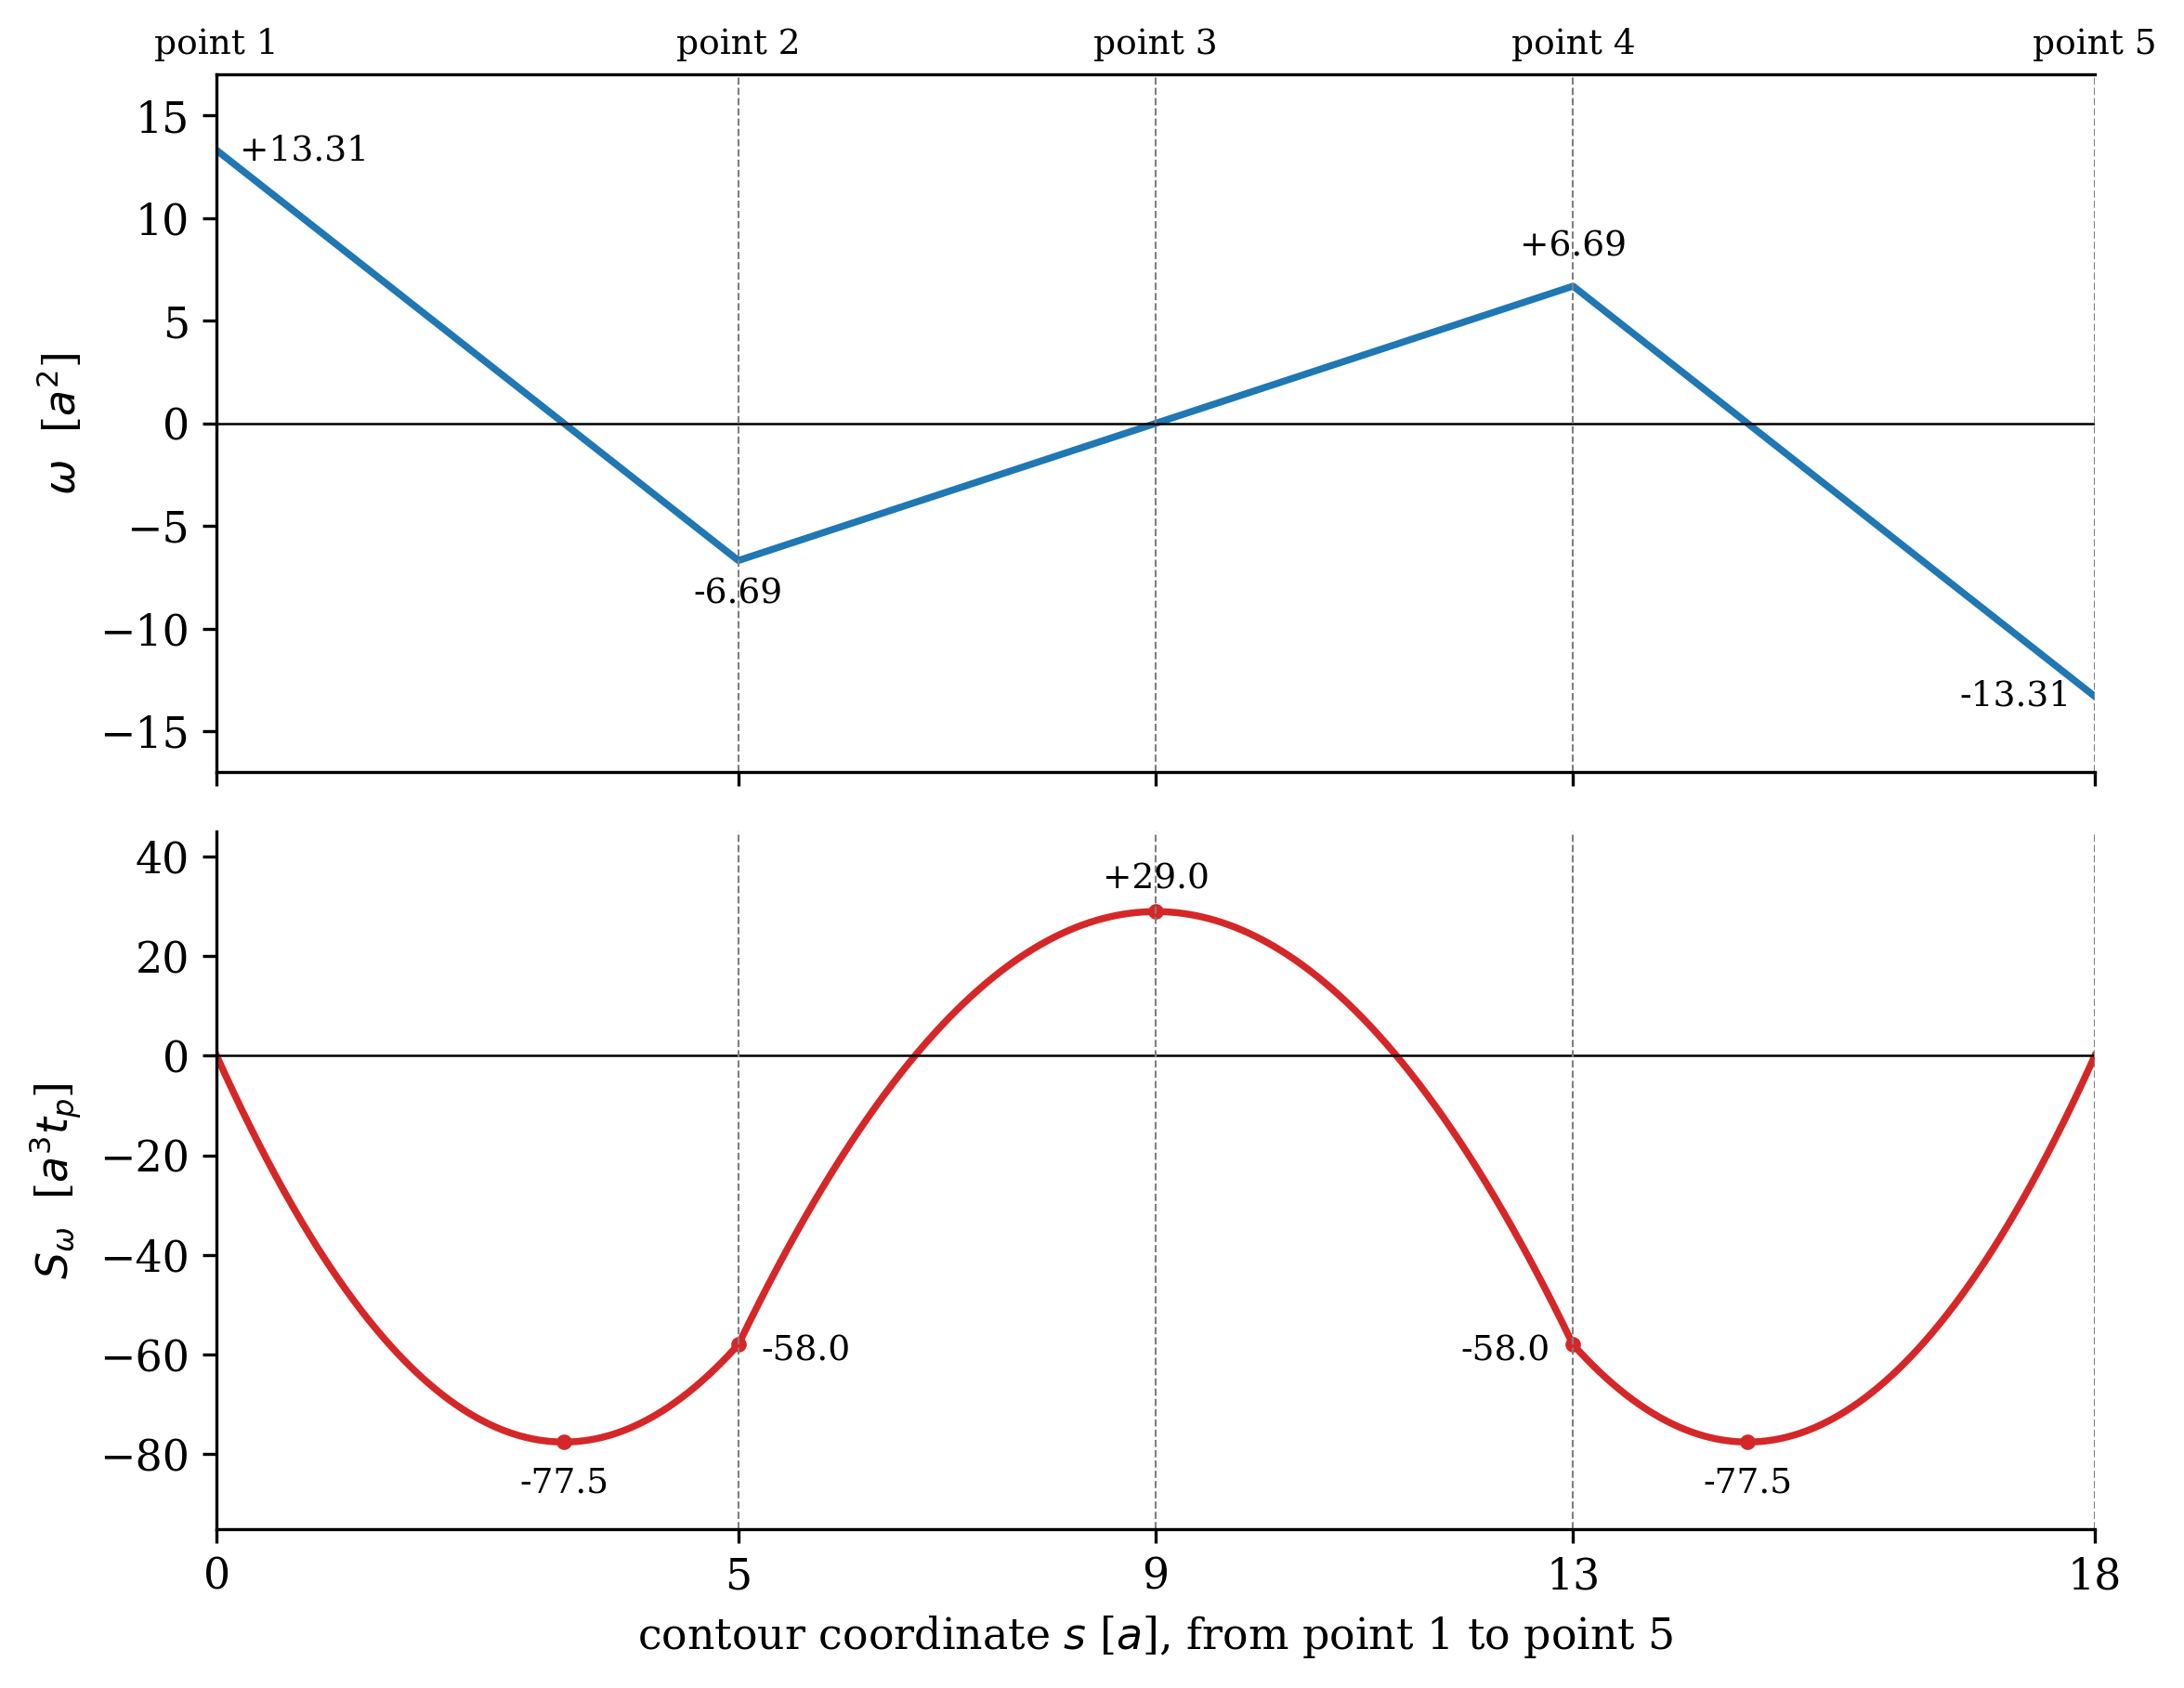
\includegraphics[width=0.85\textwidth]{figures/BU_omega_Somega_plot}
  \caption{Sectorial coordinate $\omega(s)$ (top) and sectorial area moment
    $S_\omega(s)$ (bottom) along the contour of design BU, from point 1 (top of
    the port side shell) to point 5 (top of the starboard side shell).}
  \label{fig:BU_plot}
\end{figure}

\begin{figure}[H]
    \centering
    \begin{tikzpicture}[scale=0.6, >={Stealth[length=2mm,width=1.6mm]},
        dim/.style={thin, {Latex[length=1.6mm,width=1.2mm]}-{Latex[length=1.6mm,width=1.2mm]}},
        ext/.style={very thin, gray}]
        % enclosed area
        \fill[blue!8] (-4,0) rectangle (4,5);
        \node at (0,3.3) {$\Omega = A\cdot B$};
        % plates (line width ~ thickness)
        \draw[line width=2.6pt, line cap=rect] (-4,0) -- (4,0);   % bottom
        \draw[line width=1.4pt] (-4,0) -- (-4,5);                 % port side
        \draw[line width=1.4pt] ( 4,0) -- ( 4,5);                 % stb side
        \draw[line width=1.0pt, line cap=rect] (-4,5) -- (4,5);   % hatch cover
        % shear flow (counter-clockwise)
        \draw[->, red!75!black, thick] (-1.2,1.1) -- (1.2,1.1);
        \draw[->, red!75!black, thick] (3.2,1.2) -- (3.2,3.8);
        \draw[->, red!75!black, thick] (1.2,3.9) -- (-1.2,3.9);
        \draw[->, red!75!black, thick] (-3.2,3.8) -- (-3.2,1.2);
        \node[red!75!black] at (0,1.6) {$q$};
        % labels
        \node[above, font=\small] at (0,5.05) {$t_{hp}$};
        \node[below, font=\small] at (0,-0.1) {$t_{bp}$};
        \node[left,  font=\small] at (-4.1,2.5) {$t_{sp}$};
        \node[right, font=\small] at ( 4.1,2.5) {$t_{sp}$};
        % dimensions
        \foreach \x in {-4,4} \draw[ext] (\x,-0.2) -- (\x,-1.45);
        \draw[dim] (-4,-1.3) -- node[below, font=\small] {$A = 8a$} (4,-1.3);
        \foreach \y in {0,5} \draw[ext] (4.2,\y) -- (5.95,\y);
        \draw[dim] (5.8,0) -- node[right, font=\small] {$B = 5a$} (5.8,5);
    \end{tikzpicture}
    \caption{Design BUH: the U-section with a closed hatch cover forms one closed
             cell with enclosed area $\Omega$ and a constant shear flow $q$.}
    \label{fig:BUH_section}
\end{figure}

\section{Assignment 3: Closed Cells in Sections B}
\label{app:a3}

\begin{figure}[H]
    \centering
    \begin{tikzpicture}[scale=2.0, >={Stealth[length=2mm,width=1.6mm]}]
        \tikzset{
          big/.style={->, red!75!black, line width=2.2pt},
          mid/.style={->, red!75!black, line width=1.8pt},
          small/.style={->, red!75!black, line width=0.7pt},
          stiff/.style={line width=0.8pt}}
        % T-stiffener: \Tdown{x}{y_plate}{height}, \Tup{x}{y_plate}{height}
        \def\Tdown#1#2#3{\draw[stiff] (#1,#2) -- (#1,{#2-#3});
                         \draw[stiff] ({#1-0.125},{#2-#3}) -- ({#1+0.125},{#2-#3});}
        \def\Tup#1#2#3{\draw[stiff] (#1,#2) -- (#1,{#2+#3});
                       \draw[stiff] ({#1-0.125},{#2+#3}) -- ({#1+0.125},{#2+#3});}

        % ======================= Configuration 1 =======================
        \begin{scope}[yshift=2.75cm]
            \draw[line width=1.2pt] (0,0) rectangle (5,2);
            \foreach \x in {0.833,1.667,2.5,3.333,4.167}{\Tdown{\x}{2}{0.5}\Tup{\x}{0}{0.5}}
            % shear flow (constant)
            \foreach \x in {1.25,2.917,4.583}{
                \draw[big] ({\x-0.2},0) -- ({\x+0.2},0);
                \draw[big] ({\x+0.2},2) -- ({\x-0.2},2);}
            \draw[big] (5,0.8) -- (5,1.2);
            \draw[big] (0,1.2) -- (0,0.8);
            \node[red!75!black, below] at (2.917,-0.05) {$q$};
            % torque
            \draw[->, thick] (2.5,1) ++(-30:0.3) arc (-30:210:0.3);
            \node at (2.5,1) {\small $M_t$};
            \node[anchor=east] at (-0.3,1) {(a)};
        \end{scope}

        % ======================= Configuration 2 =======================
        \begin{scope}
            \draw[line width=1.2pt] (0,0) rectangle (5,2);
            \foreach \x in {0.833,1.667,2.5,3.333,4.167}{\Tdown{\x}{2}{0.5}}
            % trapezoids: base from x0 to x0+5/6, height b/4, 45 deg legs,
            % centres at 1.25b, 2.5b, 3.75b
            \foreach \x in {0.833,2.083,3.333}{
                \draw[line width=0.6pt] (\x,0) -- ({\x+0.25},0.25) -- ({\x+0.5833},0.25) -- ({\x+0.8333},0);
                \Tup{\x+0.4167}{0.25}{0.25}
                % net flow in legs and crown (q_m - q_t), thin
                \draw[small] ({\x+0.07},0.07) -- ({\x+0.18},0.18);
                \draw[small] ({\x+0.30},0.25) -- ({\x+0.40},0.25);
                \draw[small] ({\x+0.763},0.07) ++(-0.11,0.11) -- ({\x+0.763},0.07);
                % base (q_t)
                \draw[mid] ({\x+0.3},0) -- ({\x+0.53},0);}
            % bottom plate between trapezoids (q_m)
            \foreach \x in {0.42,1.875,3.125,4.58}{\draw[big] ({\x-0.15},0) -- ({\x+0.15},0);}
            % top plate and sides (q_m)
            \foreach \x in {1.25,2.917,4.583}{\draw[big] ({\x+0.2},2) -- ({\x-0.2},2);}
            \draw[big] (5,0.8) -- (5,1.2);
            \draw[big] (0,1.2) -- (0,0.8);
            % labels
            \node[red!75!black, below] at (1.875,-0.05) {$q_m$};
            \node[red!75!black, below] at (2.5,-0.05) {$q_t$};
            \draw[very thin, gray] (2.62,0.27) -- (3.0,0.75);
            \node[red!75!black, above, font=\small] at (3.05,0.72) {$q_m - q_t$};
            % torque
            \draw[->, thick] (2.5,1.05) ++(-30:0.3) arc (-30:210:0.3);
            \node at (2.5,1.05) {\small $M_t$};
            \node[anchor=east] at (-0.3,1) {(b)};
        \end{scope}
    \end{tikzpicture}
    \caption{Shear flow for a counter-clockwise torque $M_t$ in (a) Configuration~1
    and (b) Configuration~2. The arrow thickness gives the size of the shear flow.
    The T-stiffeners are open sections and have no net shear flow.}
    \label{fig:a3flow}
\end{figure}

\begin{table}[H]
  \centering
  \caption{Net shear flow and shear stress in the walls of the closed part of configuration~2 (Question~\ref{sec:a3-4}).}
  \label{tab:a3-walls}
  \small
  \begin{tabular}{lccc}
    \toprule
    Wall & $t$ & $q_{net}$ [$M_t/b^2$] & $\tau$ [$M_t/(b^2t_p)$] \\
    \midrule
    \textbf{Deck, sides, bottom between trapezoids} & $\boldsymbol{2t_p}$ & $\boldsymbol{q_m = 0.0503}$ & $\boldsymbol{0.0252}$ \\
    Bottom under a trapezoid                & $2t_p$   & $q_t = 0.0429$     & $0.0215$ \\
    Trapezoid legs                          & $t_p/2$  & $q_m-q_t = 0.0074$ & $0.0148$ \\
    Trapezoid crown                         & $t_p$    & $q_m-q_t = 0.0074$ & $0.0074$ \\
    \bottomrule
  \end{tabular}
\end{table}

\begin{table}[H]
  \centering
  \caption{Stiffness, strength and specific values of configurations 1--3 for $b\gg t_p$ (Question~\ref{sec:a3-5}a).}
  \label{tab:a3-specific}
  \small
  \begin{tabular}{lccc}
    \toprule
     & config.\ 1 & config.\ 2 & config.\ 3 (given) \\
    \midrule
    $I_p$ [$b^3t_p$]                    & 57.1  & 58.3  & 61.6 \\
    $M_t$ [$b^2t_p\tau_{max}$]          & 40.0  & 39.7  & 36.1 \\
    $A$ [$bt_p$]                        & 38.0  & 36.6  & 36.6 \\
    $I_p/A$ [$b^2$]                     & 1.50  & 1.59  & 1.68 \\
    $M_t/A$ [$b\,\tau_{max}$]           & 1.05  & 1.09  & 0.99 \\
    \bottomrule
  \end{tabular}
\end{table}

\begin{table}[H]
  \centering
  \caption{Split of stiffness and strength between the closed and open parts (Question~\ref{sec:a3-5}c).}
  \label{tab:a3-openclosed}
  \small
  \begin{tabular}{lcc}
    \toprule
     & config.\ 1 & config.\ 2 \\
    \midrule
    $I_{p,closed}$ & $57.14\,b^3t_p$ & $58.30\,b^3t_p$ \\
    $I_{p,open}$   & $8.33\,bt_p^3$  & $4.67\,bt_p^3$ \\
    $M_{t,open}/M_{t,closed} = I_{p,open}/I_{p,closed}$ & $0.146\,(t_p/b)^2$ & $0.080\,(t_p/b)^2$ \\
    example $b/t_p = 50$ & $0.006\,\%$ & $0.003\,\%$ \\
    $\tau_{open,max}/\tau_{closed,max}$ & $1.40\,t_p/b$ & $1.36\,t_p/b$ \\
    \bottomrule
  \end{tabular}
\end{table}
